\documentclass[tikz,border=3pt]{standalone}
\usepackage{fontspec}
\usepackage{amsmath}
\usepackage{xcolor}
\usepackage{tikz}
\usepackage{pgfplots}
\pgfplotsset{compat=1.18}
\usetikzlibrary{arrows.meta,calc,fit,positioning,shapes.geometric,shapes.misc,patterns,plotmarks}
\IfFontExistsTF{Arial}{\setsansfont{Arial}}{\setsansfont{TeX Gyre Heros}}
\renewcommand{\familydefault}{\sfdefault}
\tikzset{
  >={Stealth[length=2.2mm,width=1.5mm]},
  exact title/.style={font=\bfseries\fontsize{10.5}{12}\selectfont,align=center},
  exact subtitle/.style={font=\fontsize{6.3}{7.2}\selectfont,align=center},
  exact label/.style={font=\fontsize{6.4}{7.5}\selectfont,align=center},
  exact tiny/.style={font=\fontsize{5.3}{6.3}\selectfont,align=center},
  panel/.style={draw=black!14,rounded corners=1.2mm,fill=white,line width=.45pt},
  neutral/.style={draw=black!30,fill=black!3,rounded corners=1mm,line width=.45pt},
  arrow/.style={-Stealth,line width=.7pt},
  softarrow/.style={-Stealth,line width=.55pt,draw=black!45},
  dashedarrow/.style={-Stealth,dashed,line width=.55pt,draw=black!55},
  metric/.style={font=\fontsize{5.3}{6.3}\selectfont,fill=white,inner sep=1pt},
}
\newcommand{\pill}[4]{\node[draw=#2!70,fill=#2!10,rounded corners=1.5mm,inner xsep=3pt,inner ysep=2pt,exact label,text=#2] (#1) at #3 {#4};}
\newcommand{\frameboxx}[4]{\draw[draw=#2!65,fill=#2!8,rounded corners=.6mm,line width=.5pt] (#1.south west) rectangle (#1.north east);\node[exact tiny,text=#2] at #3 {#4};}
\newcommand{\axislabel}[3]{\node[exact tiny,text=black!60] at (#1) {#2};\node[exact tiny,text=black!60,rotate=90] at (#3) {#2};}

\definecolor{sblue}{HTML}{2F80ED}\definecolor{sorange}{HTML}{F4A261}\definecolor{sred}{HTML}{E76F51}\definecolor{sgreen}{HTML}{45A06F}\definecolor{sink}{HTML}{263238}\definecolor{slav}{HTML}{F2F4F7}
\begin{document}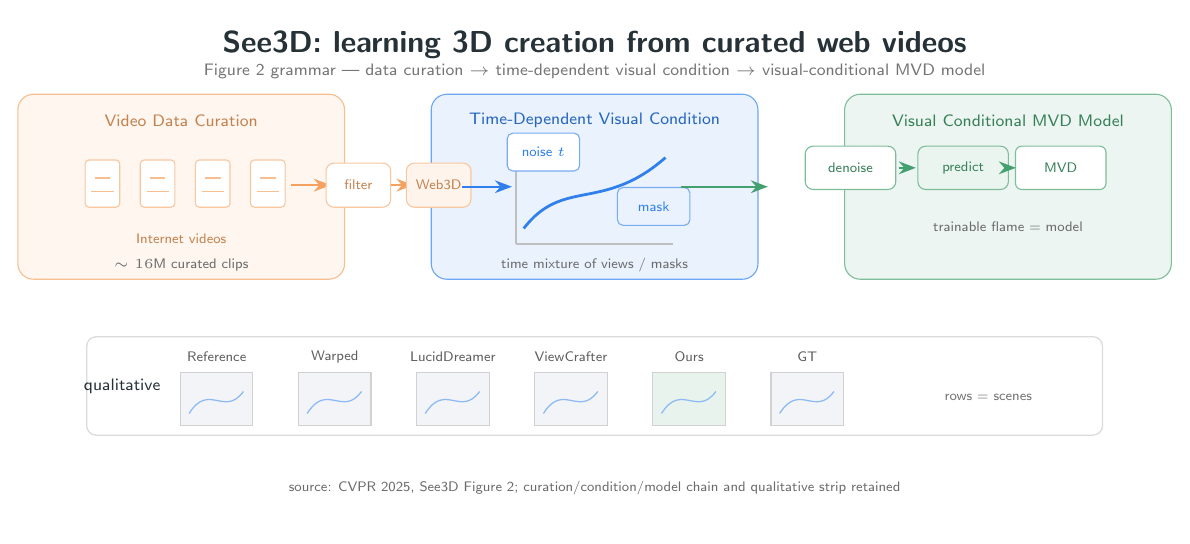
\begin{tikzpicture}[x=1cm,y=1cm]
\path[use as bounding box] (-.2,-4.0) rectangle (14.2,2.2);
\node[exact title,text=sink] at (7,1.98) {See3D: learning 3D creation from curated web videos};
\node[exact subtitle,text=black!54] at (7,1.65) {Figure 2 grammar — data curation \(\rightarrow\) time-dependent visual condition \(\rightarrow\) visual-conditional MVD model};
\foreach \x/\title/\c in {1.75/Video Data Curation/sorange,7.0/Time-Dependent Visual Condition/sblue,12.25/Visual Conditional MVD Model/sgreen}{\node[draw=\c!70,fill=\c!10,rounded corners=2mm,minimum width=4.15cm,minimum height=2.35cm] (p\x) at (\x,.18) {};\node[exact label,text=\c!80!black] at (\x,1.02) {\title};}
\foreach \x in {.75,1.45,2.15,2.85}{\draw[draw=sorange!60,fill=white,rounded corners=.5mm] (\x-.22,-.08) rectangle (\x+.22,.52);\draw[sorange!70,line width=.45pt] (\x-.14,.12)--(\x+.14,.12);\draw[sorange!70,line width=.45pt] (\x-.1,.29)--(\x+.1,.29);}\node[exact tiny,text=sorange!80!black] at (1.75,-.48) {Internet videos};\draw[arrow,draw=sorange] (3.15,.2) -- (3.65,.2);\node[draw=sorange!60,fill=white,rounded corners=1mm,minimum width=.82cm,minimum height=.56cm,exact tiny,text=sorange!80!black] at (4.0,.2) {filter};\draw[arrow,draw=sorange] (4.42,.2) -- (4.7,.2);\node[draw=sorange!60,fill=sorange!12,rounded corners=1mm,minimum width=.82cm,minimum height=.56cm,exact tiny,text=sorange!80!black] at (5.02,.2) {Web3D};\node[exact tiny,text=black!58] at (1.75,-.82) {\(\sim16\)M curated clips};
\draw[black!25,line width=.6pt] (6.0,-.55) -- (8.0,-.55);\draw[black!25,line width=.6pt] (6.0,-.55) -- (6.0,.74);\draw[sblue,line width=1pt] (6.1,-.35) .. controls (6.6,.3) and (7.1,-.15) .. (7.9,.55);\node[draw=sblue!65,fill=white,rounded corners=.7mm,minimum width=.92cm,minimum height=.48cm,exact tiny,text=sblue] at (6.35,.62) {noise \(t\)};\node[draw=sblue!65,fill=sblue!10,rounded corners=.7mm,minimum width=.92cm,minimum height=.48cm,exact tiny,text=sblue] at (7.75,-.07) {mask};\node[exact tiny,text=black!58] at (7.0,-.82) {time mixture of views / masks};
\node[draw=sgreen!70,fill=white,rounded corners=1mm,minimum width=1.15cm,minimum height=.55cm,exact tiny,text=sgreen!80!black] at (10.25,.42) {denoise};\node[draw=sgreen!70,fill=sgreen!11,rounded corners=1mm,minimum width=1.15cm,minimum height=.55cm,exact tiny,text=sgreen!80!black] at (11.68,.42) {predict};\draw[arrow,draw=sgreen] (10.86,.42) -- (11.08,.42);\node[draw=sgreen!70,fill=white,rounded corners=.8mm,minimum width=1.15cm,minimum height=.55cm,exact tiny,text=sgreen!80!black] at (12.92,.42) {MVD};\draw[arrow,draw=sgreen] (12.28,.42) -- (12.35,.42);\node[exact tiny,text=black!58] at (12.25,-.33) {trainable flame = model};
\draw[arrow,draw=sblue] (5.32,.18) -- (5.95,.18);\draw[arrow,draw=sgreen] (8.1,.18) -- (9.2,.18);
\node[panel,minimum width=12.9cm,minimum height=1.25cm] at (7,-2.35) {};
\node[exact label,text=sink] at (1.0,-2.35) {qualitative};\foreach \x/\lab/\cf in {2.2/Reference/slav,3.7/Warped/slav,5.2/LucidDreamer/slav,6.7/ViewCrafter/slav,8.2/Ours/sgreen!13,9.7/GT/slav}{\node[exact tiny,text=black!63] at (\x,-1.98) {\lab};\draw[draw=black!18,fill=\cf] (\x-.46,-2.85) rectangle (\x+.46,-2.18);\draw[sblue!55,line width=.45pt] (\x-.35,-2.7) .. controls (\x-.1,-2.3) and (\x+.1,-2.75) .. (\x+.34,-2.42);}\node[exact tiny,text=black!55] at (12.0,-2.5) {rows = scenes};
\node[exact tiny,text=black!58] at (7,-3.65) {source: CVPR 2025, See3D Figure 2; curation/condition/model chain and qualitative strip retained};
\end{tikzpicture}\end{document}
